\documentclass[utf8,english]{gradu3}
\usepackage{graphicx} % for including pictures
\usepackage{amsmath} % useful for math (optional)
\usepackage{booktabs} % good for beautiful tables
\usepackage{csquotes} % recommended by compiler
\usepackage[bookmarksopen,bookmarksnumbered,linktocpage]{hyperref}
\addbibresource{ref.bib} 
\graphicspath{{charts/}}
\renewcommand{\baselinestretch}{1.39} 

\begin{document}

%%% Title, Abstract in English and Finnish %%%
\title{Innovation in Complex Adaptive System: an exploratory study in mobile phone industry by data mining}
\translatedtitle{Title suomeksi}
\studyline{International Business and Entrepreneurship}
\avainsanat{Avainsanat suomeksi}
\keywords{complexity theory, Complex Adaptive System, Feedback Loop, Innovation Management}
\tiivistelma{Suomen kielen abstrakti.}
\abstract{Abstract in English.}
\author{Yan Pan}
\contactinformation{\texttt{yan@yan.fi}}
\supervisor{Mirva Peltoniemi}

\maketitle

%%% The start of main contents %%%
\mainmatter

\chapter{Introduction}

The utilization of complexity theory in tackling business activities serves as a holism approach to addresses the natural characteristics of complexity that cannot be solved through reductionism science. Holism emphasizes that systems and the inclusive properties should be views as a non-separable whole, and it constructs the foundation of complexity theory application in Economics and business (e.g. \cite{smuts1926holism}; \cite{auyang1999foundations}). Albeit the potentially complex structure of the modern economic world, it is not easy to deny the existence of fundamental laws. The heuristics of each market participant is generally as linear as profit maximization, but unexpected, complex, nonlinear and chaotic results may occur even in a simple law-oriented system (\cite{nicolis1995introduction}). The introduction of complex adaptive systems tackles the challenges in understanding business systems by "organization as machine" especially under turbulent environments (\cite{dooley1997complex}). In terms of innovation management, strategy and organizational form are the most popular domains, where selection-adaptation debate, resource-dependence and knowledge-learning perspective are widely discussed. 

 Innovation has long been an active business research topics. Traditionally, reductionism and determinism composed the paradigm in classical management theories, by which business outcomes can be theoretically predictable if corresponding planning, budgeting and management are conducted, for example, Taylor's (\citeyear{taylor1911shop}) management principles and equilibrium in competitive economy (\cite{arrow1954existence}). Such (semi-)machine paradigm is greatly influenced by Newtonian thoughts featuring systems laws with equilibrium. As early as 1960s, researchers have started to investigate the speed of firms' responses to new techniques. \citeauthor{mansfield1963speed} (\citeyear{mansfield1963speed}) discovered that company size and profitability influences the waiting time before the company embracing the latest technical development. This finding coincides with traditional resources-based views, where the causal relationship is relatively more concentrated in resources deciding innovations (see for example \cite{wernerfelt1984resource}). Nevertheless, traditional approaches tended to highlight certain pre-specified points of view into the hyper-competitive and highly complex markets, where the outcomes might be subject to confounding factors and confusion between correlation and causation. Hence, there is a need for learning the properties of complex systems within the business discipline. Innovation, as multi-disciplinary social phenomenon, indeed demands a complexity-based analysis with systematic views on technology, new product, diffusion, industry and macroeconomics as a whole, instead of detached components.

With an intention to create a more deliberate perspective supported by classical innovation management theories and modern complexity theory, this thesis is to accentuate both industrial and individual-level, where individuals are considered to be a minor agent in an industry with rather limiting market power and public influence. Such outlook represents Mezzo-economics approach over the organizational and managerial perspectives in the area between micro- and macroeconomics (\cite{kozuharov2011mezzo}). Supported by empirical evidence from the mobile phone industry and with a holistic approach-enabled complexity analysis, the succeeding paragraphs first pursue the complex characteristics in mobile industry in a relatively qualitative manner, and then quantitatively perceive the evolutionary pattern in the industry innovation empowered by exploratory statistics. Finally, the attempt is to present a feasible strategy in terms of innovation that is yielded from the insight towards the industrial complexity. 

In the next paragraph, a review on relevant previous researches will be presented, followed by a brief qualitative analysis on industry seeking to demonstrate the complexity concept and challenges with traditional reductionism approach. The preceding chapter then spotlights on the research object, including data, key methodology and assumptions inspired by complexity analysis. The characteristics and empirical evidence from mobile phone industry will be analyzed in the framework of complex adaptive system on the findings, addressing the complexity nature and hyper-competitive market. The thesis will be concluded with management implications and discussion on the potential improvement in utilizing the data.

\chapter{Literature Review}

\section{Complexity-Based Analysis in Economics and Management Theory}

The terminology holism defines a philosophy concept describing that parts of a whole are in intimate interconnection, such that they cannot exist independently of the whole, according to Oxford Dictionary. This thesis refers synthetic holism to a systematic thinking, where the research objects are consider as a hard-to-separate system, where the outcome is greater than the sum of each components. Multiple scientific disciplines have experienced the transformation into chaos, complexity, non-linearity and dynamical system analysis, and traditional reductionist methods shifted to complex adaptive studies (\cite{urry2005complexity}). The complexity approaches combine and enhance both system thinking and process thinking (\cite{thrift1999place}). 

One of the major research object in holistic complexity analysis is the complex adaptive system that generically characterized for self-organization, emergence, interdependence, feedback, non-equilibrium, coevolution, path-dependence and creation of new order (\cite{mitleton2003complex}). Organizational and industrial dynamics are among the top in innovation management studies. \citeauthor{jung2014structure} (\citeyear{jung2014structure}) introduced both qualitative and quantitative framework for system thinking on business dynamics, allowing simulation-based test on strategies and policies. The use of simulation distinguishes the complexity analysis from reductionism approach. The integrated business ecosystem framework highlighted the dynamic feedback loop as a consequence of conscious choice and limited knowledge among interconnected organizations (\cite{peltoniemi2006preliminary}). The framework also established the links among various business ecosystem concepts, and addresses the reasons for a non-deterministic, nonlinear and unpredictable future for organizations within the ecosystem.

In economics theory, traditional fixed point has shifted to dynamic attractors; perfect rational agents has become more realistic rational; network structures play an increasingly important role and emergent patterns are more likely to be non-linear (\cite{beinhocker2006origin}). Santa Fe Institute pioneers the complexity economics research, and has released the volume of The Economy as an Evolving Complex System (I, II and III as of 2018). The books have provided both complexity vision and relevant mathematical modelling approach, where the evolving, nonlinear and dynamic economics systems are clearly presented. In the third release, it is argued that the diffusion of innovations occur in social and/or geographic networks, and agents' innovation adoption decision is upon the combination of the economic value and local popularity of the innovation in question (\cite{young2006diffusion}). The current economy sees the need for Agent-based Modelling that diversifies the agents and clears the boundary of economics; most importantly, it eliminates the prejudice of economic equilibrium (\cite{farmer2009economy}). Classical assumptions on collective rationality has experienced huge challenges in contemporary economics. Even many social norms  in money-spending is neither collectively rational nor Pareto-efficient (\cite{elster1989social}). Therefore, diversity-emphasized agent -based economic theories have gain the popularity, and emerged to be a complement to equilibrium theories. 

Organizational change is one of the overwhelming research paths of innovation management. There are two dominate perspectives on organizational revolution with one focusing on organizational adaptation and the other environmental selection. Various early literature has suggested that two views are not conflicting but complementary and inter-related (\cite{levinthal1991organizational}). Consensus building among stakeholders has become common practice to handle environment uncertainty and complexity. The potential effects of consensus building can be categorized into 3 orders, with first order effects including the internal strategies and resources; second order focusing on coordination in perception changes; and third order leading to new intuitions and coevolution by minimizing conflicts (\cite{innes1999consensus}). In short, it can be expected that organizational affairs, stakeholders relationship management, in addition to innovation strategy itself would be strong influential factors in innovation outcome.

In brief, modern management researches and economic theories encounter a transition towards complex systems. The definition and behavior of an agent cover an increasingly large set of research topics, while the complexity-based analysis, for example complex adaptive system view and ecosystem framework, is becoming trendy and requesting more research focus.

\section{Complex Adaptive System and VUCA Environment}

Similar to a biological ecosystem in a run long, an organization is under the pressure of "innovate or die" (\cite{drucker1999knowledge}). Such pressure motivates the ecosystem participators (or agent in the context of economics) to both evolute and co-evolute. Furthermore, \citeauthor{levinthal1991organizational} (\citeyear{levinthal1991organizational}) has proposed that organizational adaptation and environmental selection are fundamentally interdependent, which had been developed from the conception of adaptation and selection where two processes are separated into their own domains (e.g. separate researches on survivals and on adaptation).

John H. Holland (\citeyear{holland1992complex}) summaries the fundamentals of a complex adaptive system as,

\begin{quote}
A complex adaptive system has no single governing equation, or rule, that controls the system. Instead, it has many distributed, interacting, parts, with little or nothing in the way of a central control. Each of the parts is governed by its own rules. Each of these rules may participate in influencing an outcome, and each may influence the actions of other parts.
\end{quote}

Evolution is one of the fundamental part in a complex adaptive system. The most common evolutionary hypothesis, under multiple disciplines, includes the paradigms of gradualism, punctuated equilibrium and catestrophism (e.g. \cite{gould1972punctuated}), describing the different shapes and patterns of collective changes in an complex adaptive system like ecosystem. While gradualism stands for a rather stably slow changes and catestrophism implying a relatively high level of unpredictableness, puncture equilibrium has been attracting business studies, from technical diffusion (e.g. \cite{loch1999punctuated}),  firm growth (e.g. \cite{mudambi2011proactive}) to organizational science (e.g. \cite{romanelli1994organizational}).

VUCA, first used to describe Volatility, Uncertainty, Complexity and Ambiguity of a general situation/environment in 1987, is an acronym that has recently emerged in business researches. The industry nature of multilevelness and non-linearity imposes a significant inertia on technology innovations partially due to (International) division of labor and expertise.

The major challenge proceeding the VUCA nature of high-tech industry is the impossibility to "stay ahead". The paradigm of innovation management, business process and industry cycle is unlikely to be simply summarized into dominant rules by virtue of the dynamics in modern world. It is barely possible for an agent, nor any other party, to assert that specific actions guarantee success. The problem of how to stay constantly competitive is indeed a wicked problem, which, abstracting from \citeauthor{rittel1974wicked} (\citeyear{rittel1974wicked}) and \citeauthor{buchanan1992wicked} (\citeyear{buchanan1992wicked}), features for:

\begin{enumerate}
    \item uniqueness and no clear definition;
    \item being multi-causal and interconnected;
    \item stakeholders have conflicting agendas;
    \item straddle organization and disciplinary boundaries;
    \item non-existence of admissible operations list;
    \item better\/worse solutions instead of right\/wrong answers;
    \item every wicked problem is a symptom of another higher level problem;
    \item long time to evaluate solution.
\end{enumerate}

The wickedness eliminates the possibilities for simple action plan that guarantees success. For example, raising the price does not surely squeeze demands; imitating a successful product does not necessarily provide any advantage nor disadvantage. \citeauthor{burnes2005complexity} (\citeyear{burnes2005complexity}) proposed alternative business strategy that could potentially serve as feasible solution, which emphasizes the interactions and feedback loops in a unpredictable system. Fundamentally, a dynamic, agile and evolutionary approach is necessary in stead of a static one.

The concept of complex adaptive system consists autonomous and interacting agents, and agents have the capability to adapt themselves to local (or individual) and global(or population) level (\cite{macal2010tutorial}). The mobile phone vendors and other industry participants, without any doubt, are autonomous in the sense of independent decision making, while significant interaction with each other persists due to technological and social reliance. The wide-sense innovation, including the innovative actions in production, usability, marketing, channels, etc., is the most important approach for agents to adapt to the environment. The highly aligned characteristics of theoretic VUCA complex adaptive system and the empirical mobile phone industry shall be discussed in the chapter that follows. 

\section{Exploratory Data Mining Applied in Business Studies}

A real set of empirical business data can include much more than two variables, and in many cases, bi-variate and multivariate exploratory analysis on the extraction of the most interesting information are necessary to evaluate the relationships, and such methods applied to both quantitative and qualitative data (\cite{giudici2005applied}). Data mining is a general terms that describes a large variety of statistical methods, from summary statistics to hierarchical inference models, while the most critical task is to apply the statistically correct, heuristically proper and numerically robust methodologies (e.g. "All models are wrong" aphorism; \cite{box1979robustness}). Considering the nature of complex systems, quantitative studies in highly dynamic and complex economical cluster such as the mobile phone industry are fairly demanding in the sense of statistical modelling and data collection. Luckily, an exploratory study on the emerging wicked problem can greatly help to enchance understanding and establish priorities for future research (\cite{shields2013playbook}).

\chapter{Mobile Phone Industry as a Complex Adaptive System}

Mobile phone industry features for its fast-moving and ever-emerging innovations. The competition landscape has greatly changed in last few years albeit the significant concentration, where two dominant vendors, Apple and Samsung, being at top of selling list for almost a decade according to IDC and Gartner market researches. Nevertheless, the development in the industry has enabled the increasing market capacity and lowered the entry barrier considerably. While the major players dominate the main-stream markets, especially in middle-to-high end, the mobile phone industry witnessed the growth of small-to-medium vendors in rewarding niche and sub-markets.

\section{Industry Complexity in the VUCA Environment}

For an individual mobile phone vendor, its innovation capacity is bounded by the availability and technical limitations of major components supplied by third parties. The quantitative part will discuss about the evolution and coevolution formed in complexity theory, aiming to address the VUCA within mobile phone industry's. As an introduction to VUCA, an interesting fact observed in the industry is first analyzed.

The mobile phone industry emerges a potentially astonishing phenomenon that top echelon executives' personal taste and ambition greatly influences the innovation development path. Monetary rewards are usually assumed to be the fundamental motivation in entrepreneurship; however, such motivation does not apply to all decision makers in mobile phone industries. A note-worthy observation is Smartisan with its CEO, Mr. Luo, who claims that the philosophy of Smartisan is the feelings. In the domain of user interaction, interface and experience (UI, UX) innovation, after years of major design trend changed from skeuomorphism to flat and material design lead by Google and Apple during 2012 to 2014 (\cite{burmistrov2015flat}), Mr. Luo insists with proud the skeumorphic design that replicating three-dimensional real world objects even in Smartisan's recent release in mid-2018. Similar actions can be observed from Smartisan product line in terms of phone shape, coloring, processing and manufacturing characteristics. In addition to the design preferences, entrepreneur's ambition would structure the development path and product line especially within an SME. 

There have been various examples that a mobile phone vendor extends its area into other consumer electronics, and the reverse is also true, for example Microsoft's ambition to expand in mobile phones. The benefits of such taste and ambition could lead to a successful niche market participant that does not pursue main-stream fashion, while the potential hindrance shall include failure in locating major market demands, negligence of major business opportunity, distracted focus and over-investment in R\&D, etc. There are various established theories discussing the correlation between organizational outcomes and executives' backgrounds, especially the upper echelons theory published by \citeauthor{hambrick1984upper} (\citeyear{hambrick1984upper}). This thesis shall not extend to (reductionism) managerial theory as such, and the evidence from mobile phone industry implies that not only managerial experiences but also other personal characteristics would have influenced the mobile phone brand. A manager may be viewed as a genius prophet or a market-blind arrogant one due to her/his ambition and preferences, whereas the impossibility of foreseeing the outcome persists until the competitive market proves it.

\begin{figure}[htb]
    \centering
    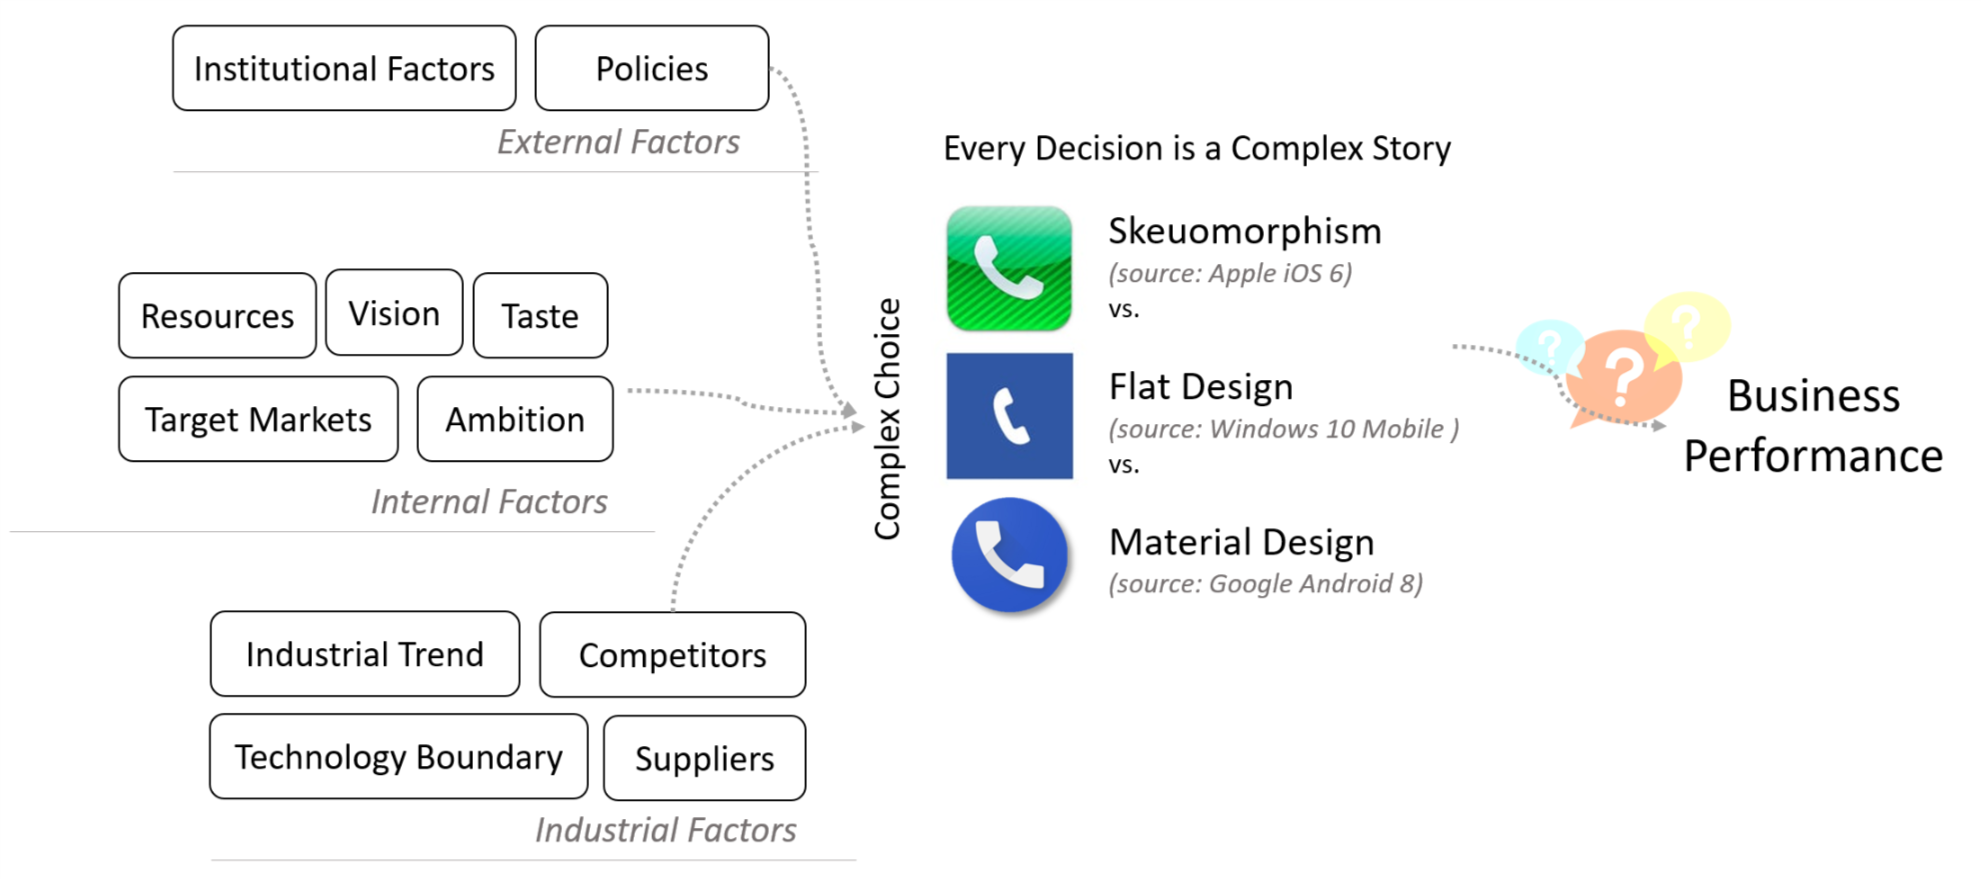
\includegraphics[width=0.99\textwidth]{design.png}
    \caption{Illustration of complexity: Skeumorphism vs. Flat/Material Design}
    \label{fig:design}
\end{figure}

While there are various factors affecting the design, structure and technical specifications of new mobile phones in micro scales (individual or a cluster of mobile phone vendors), the industry contains significant unpredictable multidirectional causality. One unique example is once again the UI/UX design, the business ecosystem does not provide an assertive answer on whether the major players, for example Apple, Samsung and Google, led the design trend or the early adoption of design trend boosted the giants in the market. Figure \ref{fig:design} briefly illustrates the complexity in user interface design.

A further layer of innovation complexity comes from the orientation of innovation. Traditionally, software user-friendliness development and hardware technology advancement are two main innovation directions in the mobile phone industry, but a trivial trend has stemmed that companies heavily leverage in user-tracking and mass-data-collection, where behavioral analysis seems to be a non-trivial task in production innovation cycles. Furthermore, subscription-based (software) cloud service seem coincide has activated the increasing need for user behavioral information, either in an ethical or unethical way. emergence of ad-supported mobile phone operating systems has further strengthened the efforts in user-tracking for precise marketing in exchange for subscription-style super-revenue/profits. 

To summarize the VUCA charateristics, \textbf{volatility} in the mobile phone industry is partially a consequent of technology innovation while it is also highly related to the frequent changes in end users’ preferences. On a given time and even in a specified market, the existence of vast variation in mobile phones design and specifications is an indication of the industry volatility. \textbf{Uncertainty} describes the challenges in foreseeing the industry trend, forecasting demands, assurance of successful R\&D progress and all other factors in supply chains, sales channels, macroeconomics in addition to manufactures themselves; succeeding paragraphs shall discuss more. \textbf{Complexity} reflects the interconnecting, nonlinear, multidimensional and multileveled network systems within the industry. \textbf{Ambiguity} mainly originates from the nonlinear causality, where one cannot simply conclude certain actions surely leads to specific results. The mobile phone with most advanced technology does not necessarily to be a top seller, and the top seller might not contain any technical highlights. Ambiguity is also partially endogenous characteristics of the industry. The boundary between mobile phones, tablets, laptops has become increasingly ambiguous, and meanwhile the technology development paths behind are rather interdisciplinary.

\section{Innovation, Evolution and Adaptation}

Innovation within an organization can be viewed as complex projects, where standardized  procedures do not usually apply due to the VUCA environment, and consequently, innovation processes are not separable nor linearly sequential in reality. Despite the "best practices" (for example, dominant design) may exist in the current market, they are not necessarily helpful in innovation strategy-making because of the fast-changing consumers' needs and ever-evolving competition. 

Evolution is non-linear sequence of differentiating, selecting/picking and amplifying, while innovation is the major source of evolution such that innovation occurs in each sub-process of evolution. Similar to the statement that gene mutation and genetic variation are essential in ecological evolution, innovation and commitments to R\&D are key for business evolution. Furthermore, evolution describes a collective population behavior and innovation is an action that an individual can undertake.

In the context of complexity theory, evolution is a common terminology describing the gradual changes in a complex system. The fundamental differences between evolution and innovation in mobile phone industry, a complex adaptive system, is that evolution precisely defines the system-wide changes and innovation serves only as a part, a necessary procedure and sometimes an outcome of evolution. An industrial evolution requires not only innovation but also the interaction among different parties inside and outside the industry system. An illustrative way to understand evolution is to view the improvement (or more precisely, change, as it may not always be superior to the previous) in mobile phones are the observable outcome of the procedures that involves technology innovation, adoption and diffusion.

\section{Assumptions and Research Questions}

Although rational behavior is commonly assumed in business studies, there is significant amount of observations indicating irrational decision and business practice in the mobile phone industry. However rationalism is always a relative term, since rationality in economics is not necessary concurrent with psychological rationality (\cite{hogarth1987rational}). The methodologies used in this thesis does not require the rational behavior assumption, and it is discovered that psychological reasoning can sometimes outweigh sole profit orientation in innovation decision-making.

Few assumptions are needed for a complex adaptive system, first of all, it is not possible nor feasible to predict the future; Second, it should be assumed that every agent is autonomous and has certain level of innovation capability; in addition, an individual agent is not likely to bottom up the whole system, implying that individual or small cluster of mobile phone vendors do not have the sufficient power to reshape the industry nor to rewrite the comprehensive rules. It should be note that these assumptions are complied with systematic complexity views and are largely realistic in the business world. Even though such properties are not generally favorable in reductionism studies, this attempt of holism-centered research seeks to accentuate the natural complexity in the mobile phone industry.

The main purpose of this thesis is to enhance the understanding of complex adaptive systems in terms of evolution with the support of empirical evidences from mobile phone industry highlighted for rapid innovations. According the above discussed complexity analysis fundamentals, the following questions are to be analyzed carefully,

\begin{enumerate}
    \item Recognize the general innovation pattern in the mobile phone industry.
    \item Identify the clustered (and/or sparse) phenomena in collective (and/or solely autonomous) innovation practice and outcomes, which can be summarized as evolutionary and co-evolutionary pattern.
    \item Locate evidence of adaptive behavior within the industry, and further extended to the evidence of organizational agility.
    \item Address the multi-layeredness, interdependence and other important complex features of the mobile phone industry.
\end{enumerate}

\chapter{Data and Methodology}

\section{Data and Information Processing}

The complexity analysis is based on mobile phone data collected from public information, with the help of popular mobile phone review websites, namely GSM Arena(www.gsmarena.com) and Phone Arena (www.phonearena.com), including 8020 types/models of wide-sense mobile phones that also include certain edge-cutting equipment like GSM-enabled tablets. The data cover the phones that had been released to the public between June 2001 and June 2018. Each phone type includes basic market information (announce date, release date, market status, etc.) and detailed technical specifications from as many aspects as possible, with 161 total measurements at ideal situation. Even with the high dimensional structure, the data is featured for its objectiveness such that neither personal nor public subjective reviews, opinions and non-machine-measurable metrics are excluded. An \texttt{R}-script is created from scratch to speed up the data collection procedure and to eliminated human errors. The script achieved the purpose of web scraping on big data in an ethical manner. Nevertheless, chances are that minor errors can be present in the phone specification data in consequence of the potentially non-cross-verified vintage sources that GSM Arena and/or Phone Arena originally referred to; favorably, the data sources are mostly peer-reviewed by the website users, limiting the potential error to minimum; ergo, the data used should be sufficiently reliable and accurate.

The great dimensionality of the data not only provides a huge potential for quantitative analysis but also arises significant challenges in terms of rigorous statistical methodologies. The properties of data prohibits the use of commonly adapted (generalized) linear regression model; such characteristics include,

\begin{enumerate}
    \item Multicollinearity in linear model for the underlying data can be expected due to correlation, which is against on the fundamental statistical assumptions. (\cite{farrar1967multicollinearity}). Clearly, many measures are either directly or indirectly linearly dependent by nature. A specific example is that the capacity of battery and screen sizes are approximately linear factors that contributes to the stand-by time and talking time. Appendix \ref{app:corr} contains the correlation matrices.
    \item The distribution of data is long-tailed, unbounded and does not follow normal distribution (for statistical definition and numeric proof, see Appendix \ref{app:normality}). Even though the observations are sufficiently large in size, the Central Limit Theorem and normal approximation cannot be applied because of the interdependence, non-random sampling and non-normal population in both theoretical and empirical evidence.
    \item Regression analysis, as a classical method, is not designed for the explosive dimensions, and the curses and blessings simultaneously occur in high dimensionality (\cite{donoho2000high}).
    \item Nonlinearity and multidirectional causality (as in the previous chapters) would invalidate the selection of dependent and independent variable, and these two industrial features could not be resolved by classical modelling.
    \item Data mining techniques are sufficient for pattern recognition with fewer statistical assumptions needed.
\end{enumerate}

The currently research utilized only a minor proportion of all available data, and the choice of dimensions are based solely on the importance and dominance of technical specifications that impact on end-user experience. Though the utilization of the full data become lower, such processing allows more reliable and informative quantitative analysis as detailed in the section below. Table \ref{tbl: vars} outlines the main data used for detailed analysis and appendix \ref{app:data summary} provides further summary statistics.

\begin{table}[ht]
\label{tbl: vars}
\caption{Data Description}
\centering
\begin{tabular}{rllrl}
  \hline
 & Description & Variable Name & Available Cases (\%) & Data Type \\ 
  \hline
  1 & \multicolumn{1}{p{3.5cm}}{\raggedright Total pixels of phone display} & the.total.pixels & 7638 (95\%) & integer\\ 
  2 & \multicolumn{1}{p{3.5cm}}{\raggedright Phone release date} & the.release.date & 3954 (49\%) & date \\ 
  3 & \multicolumn{1}{p{3.5cm}}{\raggedright Phone brand} & the.brand & 8020 (100\%) & characters \\ 
  4 & \multicolumn{1}{p{3.5cm}}{\raggedright Screen-to-body ratio in percentage} & the.screen2body.percent & 5791 (72\%) & numeric\\ 
  5 & \multicolumn{1}{p{3.5cm}}{\raggedright Group of total pixels} & the.total.pixels.group & 7638 (95\%) & categorical \\ 
  6 & \multicolumn{1}{p{3.5cm}}{\raggedright Manufacture of phone core processor} & the.systemchip.brand & 2786 (35\%) & characters \\ 
  7 & \multicolumn{1}{p{3.5cm}}{\raggedright Phone weight in gram} & the.weight.gram & 6845 (85\%) & integer \\ 
  8 & \multicolumn{1}{p{3.5cm}}{\raggedright Camera resolution in megapixels} & the.camera.megapixels & 6856 (85\%) & numeric\\ 
  9 & \multicolumn{1}{p{3.5cm}}{\raggedright Phone RAM-memory size in gigabytes} & the.ram.gb & 3945 (49\%) & numeric\\ 
  10 & \multicolumn{1}{p{3.5cm}}{\raggedright Theoretical stand-by hours} & the.standby.hours & 5846 (73\%) & numeric \\ 
   \hline
\end{tabular}
\end{table}

Screen pixel is calculated by the product of screen resolutions (e.g. full HD resolution $1920\times 1080 = 2,073,600$ in pixels), measuring the visual standard of a phone display; the large number indicates a better quality given the same screen size. The available run-time RAM-memory provides the phone high speed storage to perform tasks, and the larger number the better performance in general. Other variables are straightforward by definition.

Except for necessary data type correction and formatting, there is minimal manipulation towards the originally collected one. However, manual classification has been introduced to screen pixels in order to better illustrates the trend and to be compatible with rapid changes. 5 groups are created with regards to the original observed values in screen pixel, namely (1) greater than 4 million; (2) 1.5 to 4 million; (3) 0.8 to 1.5 million pixels; (4) 0.3 to 0.8 million pixels; (5) less than 0.3 million pixels, where almost none observed values lies on the boundary.

\section{Methodology}

The research mainly utilizes data mining approach, where bi-variate and multivariate exploratory analysis on quantitative data serves a major role to illustrate the findings within the context of complex adaptive systems. Unlike commonly adopted (generalized) linear regression methodology, the hybrid approach used in this thesis mainly relies on the non-parametric methods that reflect the nature of complex analysis by laying more emphasis on facts and market behaviors instead of causal modelling, and furthermore, they are fully compatible with data properties. In addition to the challenges in data properties, another issue exhibits in missing values. The complete cases (with all 161 dimensions available and valid) are technically 0, and even with the focused subset (11 processed dimensions) the complete cases only counts for 10.8\%. This problem is minimized by utilizing available case analysis, using all available data in a given statistical context. A specific application is using all non-missing mobile phone screen resolution when analyzing the quality of display, but the set used for this analysis can be different from the set for evaluating phone stand-by time. Given the data described, available cases analysis has significant merits over complete case analysis (e.g. \cite{kim1977treatment}) at possible cost of consistency. Further discussion on missing data handling can be found for example \citeauthor{little2014statistical} (\citeyear{little2014statistical}) and \citeauthor{pigott2001review} (\citeyear{pigott2001review}), and it is beyond the domain of this thesis.

The data collection procedure, data processing and quantitative analysis is implemented using \texttt{R}, a popular statistical programming language, and the \texttt{R}-package \texttt{dplyr} (\cite{dplyr}) greatly ease the task of data manipulation, and \texttt{ggplot2} helped creating the visualization.

\chapter{Findings}

\section{From Innovation to Evolution}

\begin{figure}[htb]
    \centering
    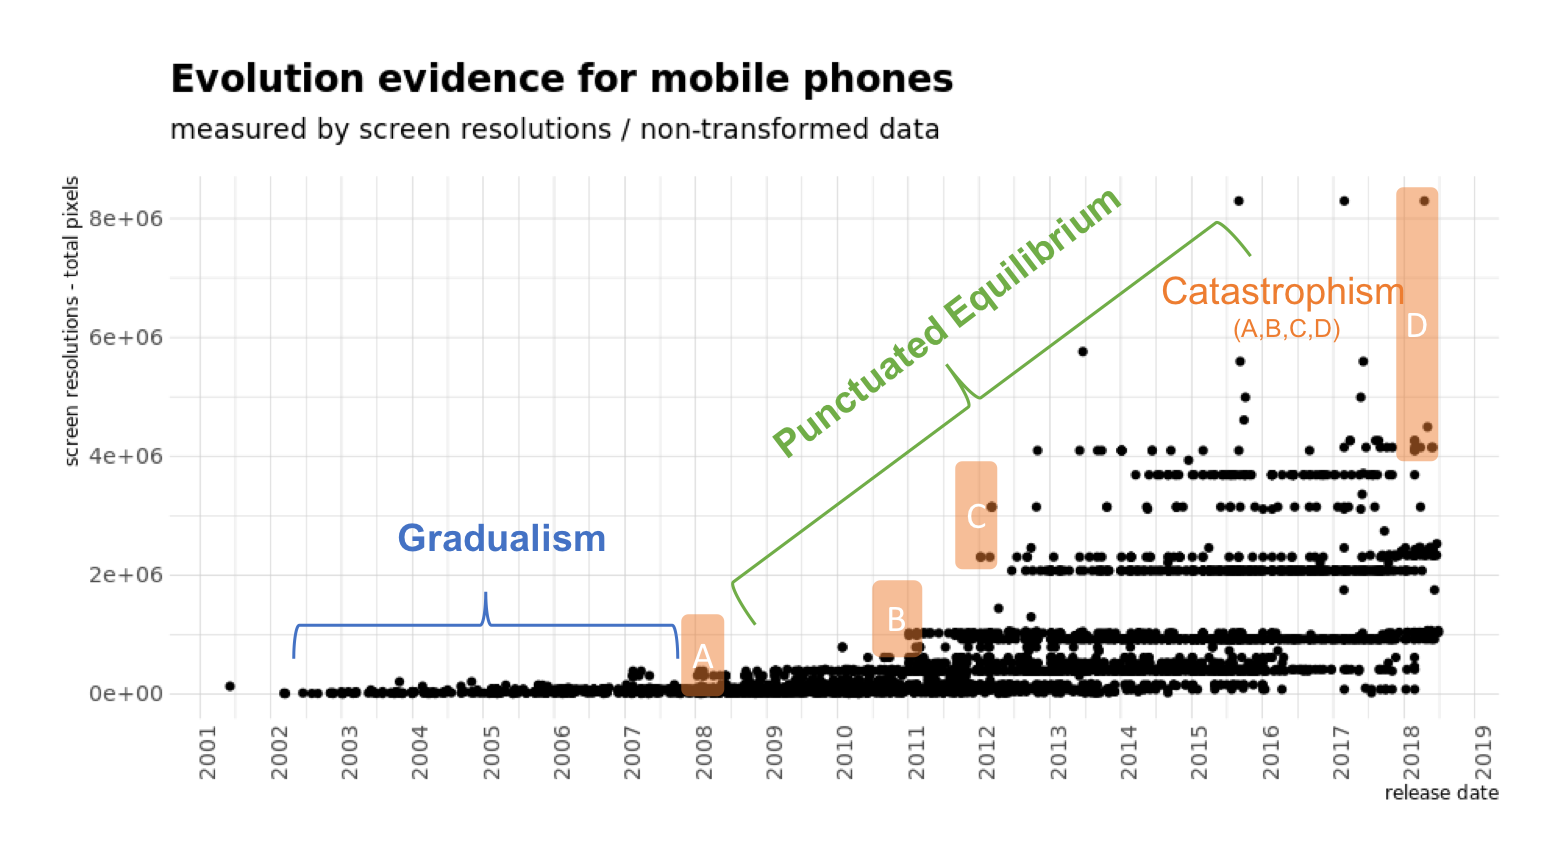
\includegraphics[width=0.99\textwidth]{evo.png}
    \caption{Evolutionary Evidence in Mobile Phone Industry}
    \label{fig:evoMethods}
\end{figure}

The evidence suggests that all 3 well-known evolutionary hypotheses, namely Gradualism, Punctuated Equilibrium and Catastrophism are simultaneously valid in mobile phone industry, as described in Figure \ref{fig:evoMethods}. Pre-2008 era exhibits a clear gradualism evolution, and the variations are small; extreme values are few and the numerical range (maximal minus minimal value) is narrow. From 2009 to 2018, the industrial generic landscape is punctuated equilibrated, within which a large-scale improvement occurs after a few year (usually in a 3-year interval, but the change occurred "faster than usual" between late-2010 and late-2012). Attention is needed for the labeled observation block, where catastrophism process better descibes the innovation outcome. In 2007, the first "catastrophe" (refer to sudden, unplanned and large-scale changes) marked with letter A took place without a sudden evolution to the whole industry, while later in 2008, the similar improvement was truly a game changer. Events labeled B in Figure \ref{fig:evoMethods} attracted a large number of followers at essentially no time, though the motivation for such change did not seem to be vigorously shaped by external factors. Obviously, customers' demands of high resolution screens had not be present before the very first such phones (the game changers) emerged to the market. The common feature for observations labeled C and D is that the evolved candidates are not limited to a single type. At similar time, the "catastrophic" event led the industry to a state of multiple simultaneous key designs, among which specifications varied incredibly much and none of sole design was dominant. 

\begin{figure}[htb]
    \centering
    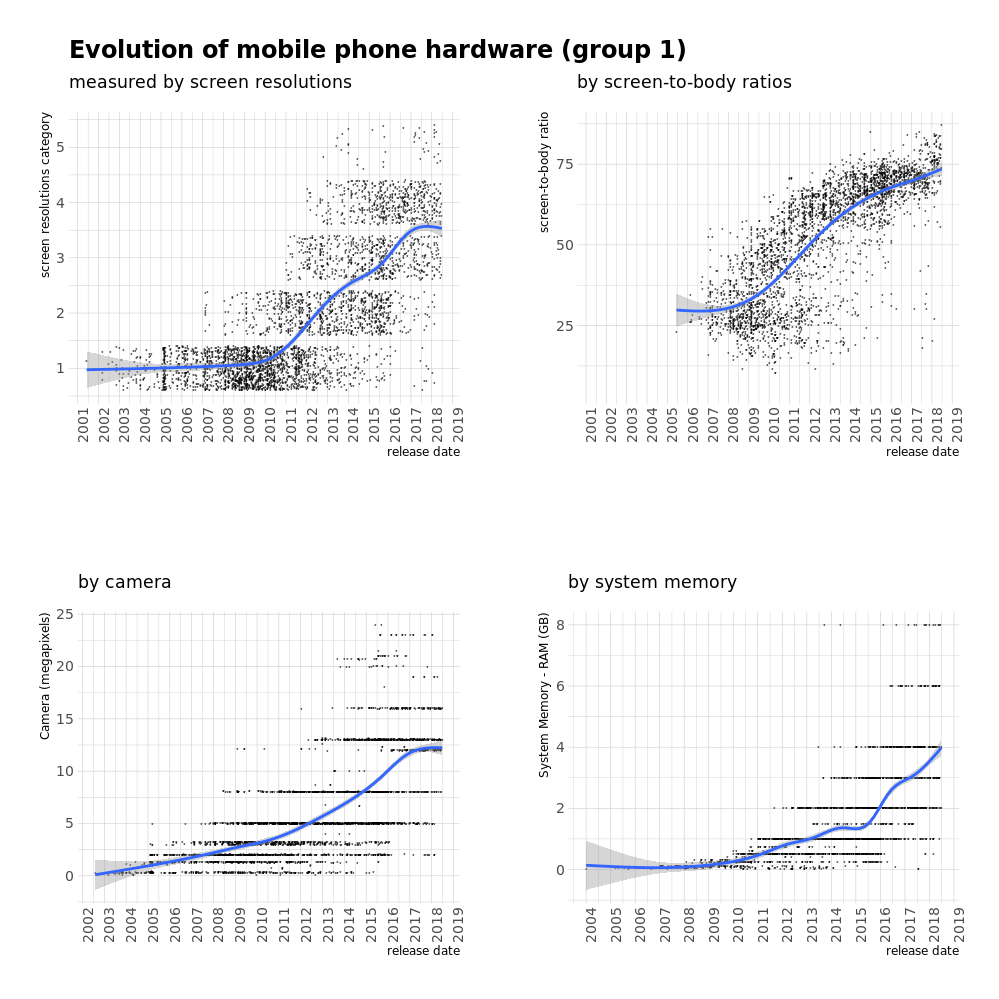
\includegraphics[width=0.90\textwidth]{evo1.png}
    \caption{Development of Hardware - Characteristics Group 1}
    \label{fig:screen resolutions}
\end{figure}

The trend of display-screen technical development illustrated in Figure \ref{fig:screen resolutions} (statistical details elaborated in Appendix \ref{app:stats note}) demonstrates an industry-level selection-adaptation process, where the dominate designs change over a long run but persists during a fixed time-series window, and it demonstrates graphically the concentrated clusters. Simultaneously, there are still non-negligible outliers present in both charts of Figure \ref{fig:screen resolutions}, especially in the lower-right corner, indicating the existence of agents that insist in producing on relatively out-of-mainstream-fashion mobile phones, either to focus on niche-market or to execute on some other concepts with complex backgrounds. Nevertheless, it is crucial to understand that causality cannot be determined through the observations, especially from a systematic view in complexity theory. While selection-adaption describes the relative dominate design phenomenon, logical causation of such can include cooperation, imitation, technology limitation, cost-price and supply-demand equilibrium and etc. 

\begin{figure}[htb]
    \centering
    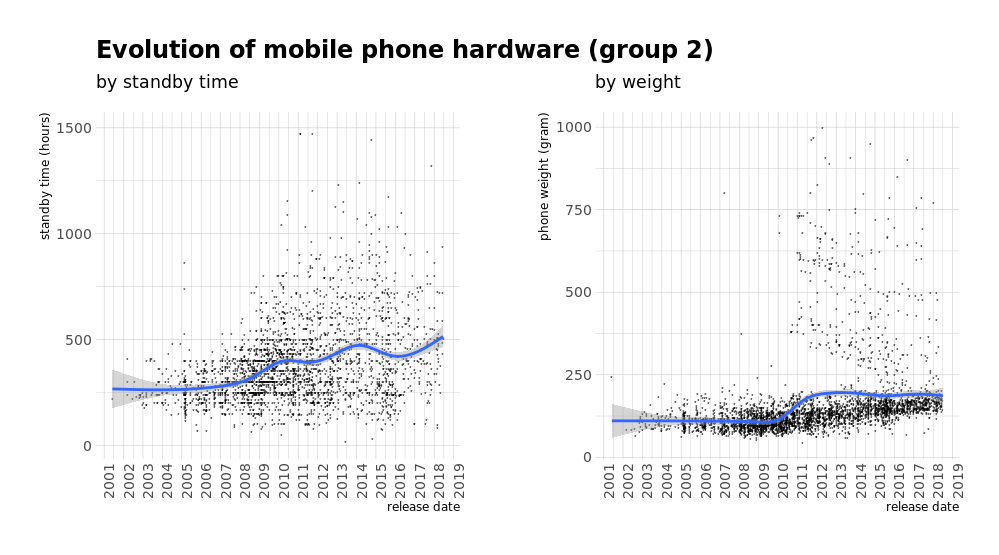
\includegraphics[width=0.90\textwidth]{evo2.png}
    \caption{Development of Hardware - Characteristics Group 2}
    \label{fig:standby}
\end{figure}

In contrast, different measurements seem to return conflicting impression as in Figure \ref{fig:standby}. While clustering and concentration is still present, the improvement seems to be absent in the long time span of 18 years. Mobile phone screens, cameras and processing memory have experienced constant punctured equilibrated innovation, but the pattern for the standby time and phone weight seem to be rather flat. Heuristically, it is a flagship phenomenon of business complexity in that dominating rules are non-existent. Asserting from Figure \ref{fig:standby}, the industry is merely motivated for prolonging standby time and lowering the weight. The few scatters in the figure suggesting that minority is cultivating in these two fields, but unlike screen and camera, such improvements has never drawn appreciation from the supplier-side (mobile phone vendors). Ironically, it is clearly not reasonable to assume that consumers do not enjoy light-weighted and long-lasting mobile phones. Explanation to such contrast between Figure \ref{fig:screen resolutions} and Figure \ref{fig:standby} can be balancing innovation inputs and rewards, and the "hidden" industrial perspective can include the industry-level co-evolution, selection-adaptation process and feedback loops. Thereupon, co-evolution provides a network-based framework to further study the interactions and explain the observed data patterns.

\section{From Evolution to Co-evolution}

The investigation into mobile phone industry reveals that most technology advancement is achieved through cooperation between mobile phone vendor and component suppliers. The diversified roles of countless business entities in the mobile phone industry compose the interconnected, interdependent, interactive, dynamic and multileveled networks, or more precisely complex networks of complex networks. The multileveled characteristics can be observed as straightforward as to classify the industry participants to either component supplier, mobile phone vendor or distribution-sales channel. This paper intensifies on the first two levels due to the objective being innovation and evolution study. Meanwhile, other systematic views can be applied to construct the multiple levels. The varied end-markets allows people to categorize the industry into high-end, middle-end and affordable segments, where interconnection are tighter within segments and looser between.

Innovation in mobile phone industry is featured for the mutual learning within networks, which in turn leads to the evolutionary phenomenon within the industry in terms of technology advancement. Among mobile phone vendors, companies tend to get inspired by their competitors. Recently, the unique non-standard edge-to-edge display with notch was initiated by Apple with iPhone X, and such screen has become rather popular despite its oddness and controversy. Industry-wide learning can be observed clearly in mobile phones as final products from the technical specifications. The multidirectional and multidimensional learning raise the complexity of the networks(s). There does not seem to be evidence that vendors from a certain tier are always learning from ones from a higher or lower tier, i.e. Apple as a high-tier mobile phone vendor is the first-mover in notch display but it indeed learned the idea of bezel-less and border-less display from others (according to the data used in this paper, the first mover seems be Essential Phone back to 2016, led by an individual entrepreneur)

\begin{figure}[htb]
    \centering
    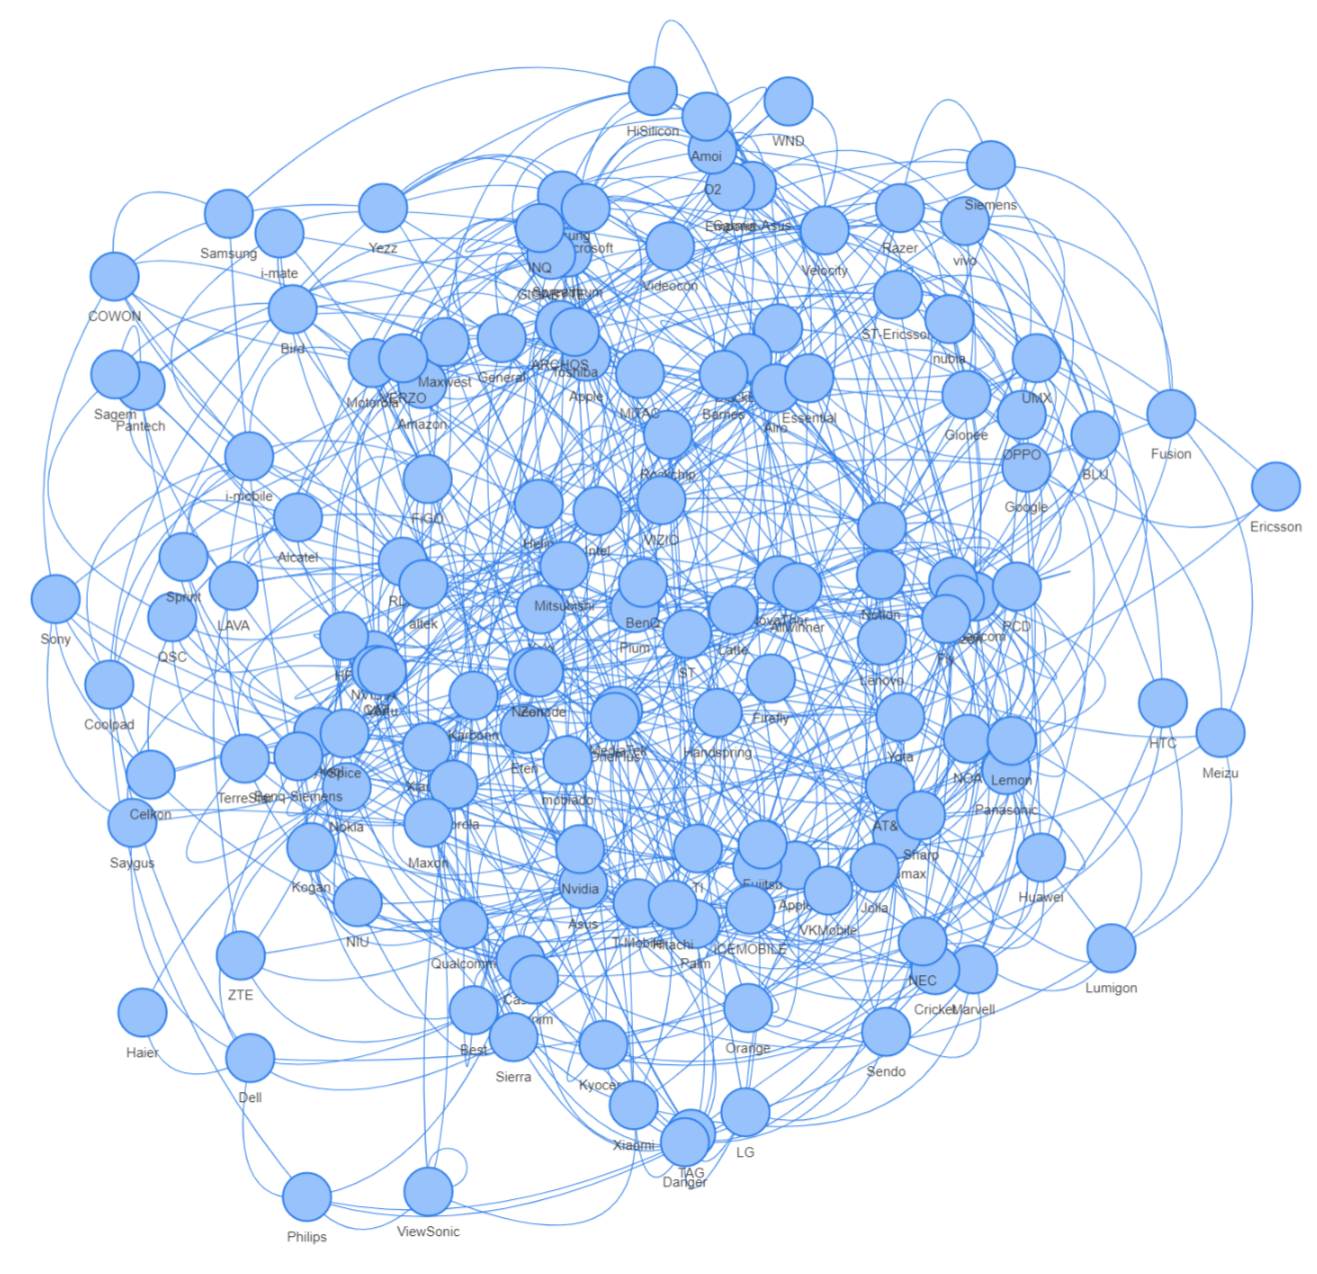
\includegraphics[width=0.88\textwidth]{network.png}
    \caption{Illustration of Complex Networks in Mobile Phone Industry}
    \label{fig:networks}
\end{figure}

Another industrial empirical fact is that one company can experience rise and fall over a relative long period, say over a decade. Technology innovations usually benefit users and bring positive features improvements, but in the context of evolution, the adoption of such innovation into the end-user mobile phones does not necessarily applause the consumers. Thus, a company may gracefully fail due to unsuccessful attempt to deliver innovation, while it may recover the situation and win the market as a consequent of another winning strategy. In this paper, later discussion on feedback loops will attempt a modern complex paradigm that explains the phenomenon of "graceful failure + recovery".

The collected data-set clearly indicates a rather limited-sized supplier market, with only about 21 brands of system chip suppliers among 2786 different major models total market and might even incur a oligopoly tendency, as demonstrated in Figure \ref{fig:systemchip}.

\begin{figure}[htb]
    \centering
    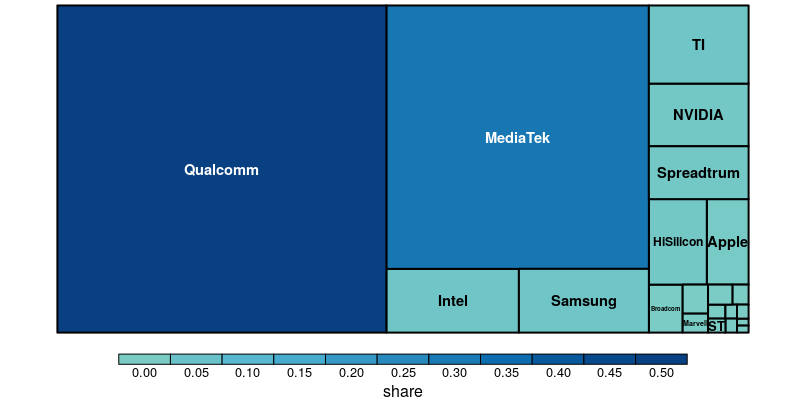
\includegraphics[width=0.85\textwidth]{systemchip.png}
    \caption{Market Share of System Chipset by Brand}
    \label{fig:systemchip}
\end{figure}

Agents in mobile phone industry, including component suppliers, mobile phone vendors and other players in different channels, are highly interconnected and interdependent to each other. In the language of network graph, each nodes are connected by many edges. Combined with qualitative sources, the interdependence can be observed at least from the following aspect:

\begin{itemize}
\item Mobile phone vendors have been \textbf{actively learning} from each other in terms of innovations in technical specifications and design concepts. Such learning includes but not limited to imitating, cooperation, partnership, mergers \& acquisitions, multiple brands strategy, and even plagiarism \& copycat. Generally, there is no single learning pattern within the mobile phone industry;
\item The roles of a single agent are usually not limited to one. The \textbf{multifunctionality} of a single entity has become more and more popular. A mobile phone vendor, in addition to manufacturing the end-market phones, is active in software design, component hardware (noticeably core processor, mobile architecture) development and even print, packaging and logistic technology;
\item Technology diffusion is \textbf{multidirectional and nonlinear}, following an evolutionary phenomenon. Traditional specialized component suppliers not only lead the technology innovation but also are influenced or pressurized by other industry participants. The transformation from a specific technical invention into materialized end-market product has to experience a complex procedure that involves a large number of companies;
\item Supply chain is critical in mobile phone industry. In various domains/sub-industry, there are rather limited number of active business entities, and due to the modular structure of mobile phones, every vendor ought to establish a stable \textbf{cooperation} with component suppliers. Meanwhile, component suppliers may be themselves mobile phone vendors (e.g. Samsung, LG). Additionally, there are strong evidences indicating the concentration in processor, display, RAM manufacturing, as well as final assembling. Therefore, the varied density in different areas of mobile phone industry arises the \textbf{uneven competition}, which increases the level of complexity.
\end{itemize}

The network with strong interdependence greatly raises the complexity of action - consequence relationship. As illustrated in the networks as shown in Figure \ref{fig:networks}, the high-level non-directed connections between nodes result in a nonlinear causal system, where it is barely possible to foresee the system responses from an action conducted by an agent. In mobile phone industry, the partners' responses, consumers' decision and competitors' strategy cannot be analytically predicted; in fact, with emergence takes place continuous in the system, whether the emergence is a technical innovation, an entrant to the industry or an abstract concept in designing the future product, the mobile phone industry persists dynamics involving countless causes and effects in the business. Unfortunately, cause and effect are not usually distinguishable in such a dynamic nonlinear system as discussed in early examples. The traditional reductionism analysis on what actions is proper given some conditions would not serve well for an agent in decision making. Instead, system thinking is necessary to cope with the complex adaptive system. Luckily, feedback loops have received considerable attention recently, and the system thinking shall solve the fundamental problem in business, i.e. what to do to survive in the mobile phone industry.

\section{The Hidden Layer: Feedback Loop and Agility}

Recall the graphic pattern in Figure \ref{fig:evoMethods} and Figure \ref{fig:screen resolutions}, and the clusters are obvious, where collective technical advancements occurs. The previously discussed innovation in terms of mobile phone screens (Figure \ref{fig:screen resolutions}) demonstrates 5 major feedback loops that pushing the industry to offer its consumers higher screen resolutions, while each agent learned to improve phone screens from its partners and competitors together with consumers' feedback. Reference to the nature of mobile phone industry and complexity theory, heuristically, an abstract evolution mechanism - the indefinite feedback loop that includes learning, (co-)evolution and feedback can be illustrated as in Figure \ref{fig:feeback loops}.

\begin{figure}[htb]
    \centering
    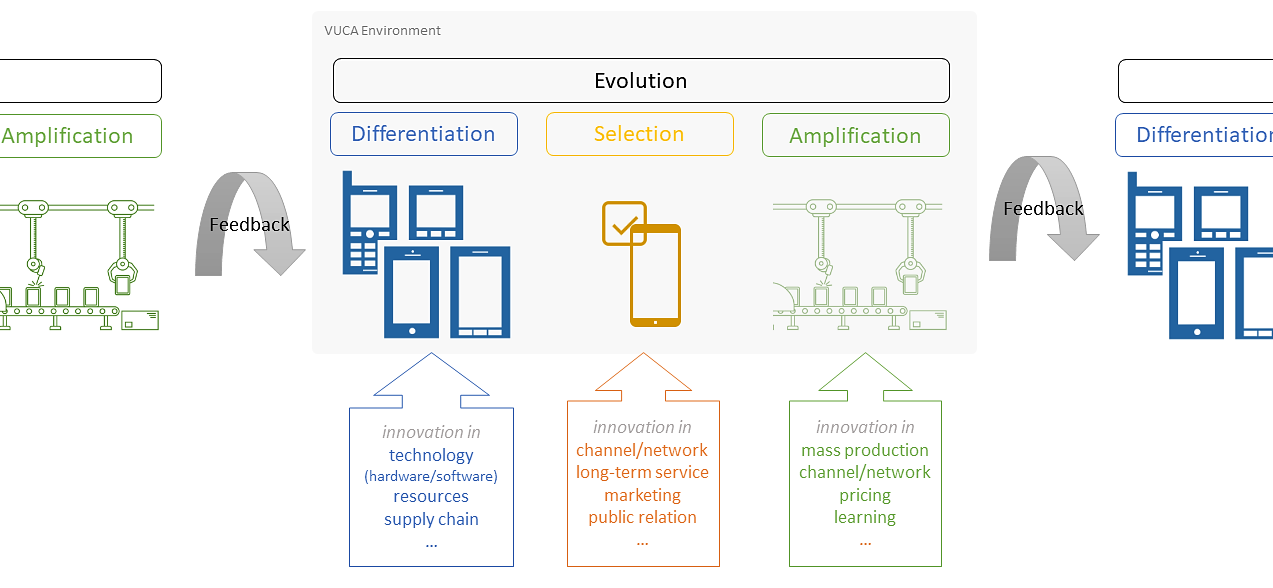
\includegraphics[width=0.99\textwidth]{feedback.png}
    \caption{VUCA, Evolution and Feedback Loops}
    \label{fig:feeback loops}
\end{figure}

Feedback is composed of two major parts in addition to a few trivial factors. Observations from mobile phone industry suggest consumer's preferences and competitors' latest innovations being the dominate sources of feedback, where the clusters of points are good indicators; meanwhile, inferences from relevant industries also provides inspiration and/or pressure, noticing graphic processor development from personal computer industry as an example.

Despite the industry being a complex adaptive system, the feedback loop clearly exists and has become a major sources for industry shift. The feedback loop draws attention to the importance of adaptation, where each agent are faced with the challenge of "adapt or die" or more commonly refer to "innovate or die". In the complex adaptive system, it can be concluded from the empirical evidence that innovation is a common and usually effective way for an agent to attempt adaptation. 

\chapter{Implications}

The findings suggest that theoretical management challenges are aroused from wickedness in VUCA environment, while the feedback loop could guides a solution. An unfavorable situation is that responses to the feedback are not always correct. It may not be a great challenge to recognize the popular design at the time being; whereas, predicting the next market-winning design by implementing accurate innovation for the next product seems to involve enormous uncertainty, which is common in the complex system. The observation of gracefully failing and recovering is one unique phenomena as a result of such unpredictableness. Graceful failing is a result of failure in materializing a correct responses towards certain system feedback or the misjudgment on the industry trend. Meanwhile,  continuous ignorance of feedback would lead to unrecoverable situation, and finally become "awkward failing" that ends into a disaster.  

Due to various unpredictableness, speed to response has thus become a most important factor inside the feedback loop system. Mobile phone industry requires its agents to be fast in both understanding the market responses and undertaking actions accordingly. Researches have discovered that innovation strategies are bounded by great variety of endogenous and exogenous factors, from resources, organizational structure to policies and institutional effects. Whereas, there is barely any inertia that prevents effective response speed. A successful company is not the one that never makes "mistakes", as they are to some extent inevitable. Rather, how quickly one can "fix mistakes" (by delivering proper products with innovation) decides how long success can last, and eventually secures sustainable business.

Practically, adaptation is the goal of an mobile phone industry agent, and meanwhile speed of response ought to be a major operational focus. The industry complexity, especially interconnectedness and multileveledness, derives the huge challenge, if there were possibility, to stay visionary on the correct trend without a continuous effort to monitor and response to system feedback.

In a brief conclusion, adaptation should be of higher priority in innovation decision making compared with predication for an ordinary agent within the complex adaptive system. A game changer in mobile phone industry can be as seldom as 1 or 2 per decade, and underlying innovation strategy were adventurous and even reckless, which exceeds the financial strength, network scale and innovation capacity in normal circumstances.

With a focal point on feedback loops, high level of agility is desirable for all agents, and meanwhile the organizational agility is a general requirement for almost all agents in the mobile phone industry. In organizational studies, agility is often referred as a synonym for flexibility, though two terms are not exact (\cite{teece2016dynamic}). In a VUCA environment under complexity theory, the patterns from empirical data cannot be achieved with the following aspects in terms of organizational agility,

\begin{enumerate}
\item \textbf{Willingness to change} is a prerequisite for agility; 
\item \textbf{Capability to innovate} is the set of practical tools to implement agility;
\item \textbf{Commitment in monitoring feedback} is the process to recognize the needs for changes, and it also states the "correct" direction for changes;
\item \textbf{Organizational dynamics} describes the internal resources that supports agility, including but not limited to, human resources, patents, networks and operating strategies. 
\end{enumerate}

For agents in the mobile phone industry, a high technology industry, resistance to change is seldom, but it may exist in both large corporate and in SMEs. In large scale companies, the resistance can arise from for example organizational bureaucracy and heavy historic burdens, while in SMEs may possibly become change-resistant due to CEO's narcissism, extreme limitation in resources etc. Innovation capability are fundamental components of agility, and such innovation can apply not only to products but also organizational efficiency, productivity and quality, as well as innovate the networks. In fact, the complex adaptive system structure demands a much wider portfolio of innovation, where evolution of networks, cooperation and organization should attract more attention. It should be noted that \textbf{network} is defined as a part of organizational agility. Organizational dynamics is relatively a vague term that urges agents to be always prepared for sudden change, and compared with innovation capacity, dynamics extends to organization behavior, strategic management, and stakeholders’ relationship management. More specifically within the mobile phone industry, the current market urges the agility in capitalization (to financially secure innovation process) and the flexibility in balancing economy of scale (internal factor) and consumption needs (that are relatively external).

Presence in a VUCA environment require all agent to understand and be capable to tackle various external factors in addition to internal process \& strategy management. A high level of organization agility thus become a wide-sense solution when faced with highly dynamic markets that are a mixture of social, cultural and nature-environmental factors.

Modern organization researches provide potentially feasible and preferable structures in terms of agility. Especially observed in the mobile phone industry, it has been indeed pioneering the organizational innovation. The online-based smart phone brand is a unique pattern symbolized for its major (if not sole) focus in online business and partner distribution networks, and in many cases, they should not even be categorized into manufacturer, as those brands are usually deeply leveraged in outsourcing. Meanwhile, their intensive reliance on the suppliers, assembling factories, distributors, marketing partners, venture capitals and influential direct clients indicates the dominating necessity for network management, in which innovation has been, and should be persist.

The complex adaptive organization is a conclusive terminology to describe the preferable structure in a complex adaptive system, and the organizational agility is the key indicator for being complex-adaptive-ready and even crisis-ready. Apparently, there is no static way to promote organizational agility since agility itself is truly dynamic. Nonetheless, a set of strategy that closely monitor the environmental feedback become one kind of positive "attitude" to adapt oneself, either a manager or an agent, to the VUCA environment. Negligence of feedback will almost surely leads to a long-term failure, though exception may exist in a short time-span. The speed of response distinguish the level of success.

\chapter{Discussion and Conclusion}

Above paragraphs have demonstrated the natural complexity in the mobile phone industry, where each agent is supposed to strive for adaptation. Data mining into the big data of vast mobile phone specifications demonstrated a few insightful patterns, including the collective behavior and clear outliers. From feedback loops, timelessness response is the key for competitive edge. Therefore, an adaptive, responsive and flexible innovation strategy and associating organizational structure would be of tremendous importance. Despite the complex causal relationships, deeply connected networks, unpredictable and unstable markets, the Figures from empirical evidence at least implies that there exists a way to survive the industry and conquer the market by continuous efforts in monitoring the feedback and commitments to address a timeless innovative solution. 

This hybrid-quantitative study presented a complexity theory view towards the innovation-evolution in mobile phone industry. Industry-level complexity has been examined carefully from the observed innovation outcomes, i.e. the mobile phones available in the market. The feedback loops, evolution paradigm and adaptive system may apply to related industries (wearable, personal computer, cloud software service industry etc.), as well as other highly dynamic industries, for example automobile industry especially the electric car segments. 

In innovation management theory, reductionism paradigm is and will be popular due to its strong and clear focus on action-result relationship. complexity theory view does not seek to replace the traditional and dominating theories, but serves as an supplementary view that emphasizes the systematic industry structure and aims to draw managers' attention to the networks and ultimately the feedback loops.

While exploratory statistics and pattern recognition sufficed to answer the research questions, the quantitative methodology is indeed comprised because of the data characteristics. The complexity theory view itself invalidates vast majority of common statistical assumptions, especially in normality, robustness and homogeneity. However, latest researches in statistics, for example network modelling and long-tail distribution would be helpful. The significant challenge of missing data potentially harmed the depth of statistical methods by invalidating principle component analysis that could have use all variables. Proper imputation for the missing values would help developing model-based quantitative methodologies, such as Agent-Based Computational Economics (ACE) framework that is specialized in modelling complex adaptive systems paradigm (\cite{tesfatsion2003agent}). Apart from business and economics research, the study of VUCA environment and complex system has developed to be multidisciplinary as computational social science and information technology has significant impact under the topic of complexity theory.

\printbibliography

\appendix

\section{Selected Data Summary}
\label{app:data summary}
\begin{verbatim}
 the.total.pixels  the.screen2body.percent the.weight.gram 
 Min.   :     96   Min.   : 4.90           Min.   :  42.0  
 1st Qu.:  38720   1st Qu.:30.11           1st Qu.:  95.0  
 Median :  96000   Median :52.45           Median : 120.0  
 Mean   : 471940   Mean   :48.82           Mean   : 143.4  
 3rd Qu.: 518400   3rd Qu.:65.77           3rd Qu.: 150.0  
 Max.   :8294400   Max.   :87.04           Max.   :2650.0  
 NA's   :382       NA's   :2229            NA's   :1175    
 
 the.camera.megapixels   the.ram.gb     the.standby.hours
 Min.   : 0.100        Min.   : 0.004   Min.   :  10.0   
 1st Qu.: 1.300        1st Qu.: 0.500   1st Qu.: 216.0   
 Median : 3.200        Median : 1.000   Median : 300.0   
 Mean   : 4.768        Mean   : 1.258   Mean   : 352.1   
 3rd Qu.: 8.000        3rd Qu.: 2.000   3rd Qu.: 432.0   
 Max.   :41.000        Max.   :16.000   Max.   :3000.0   
 NA's   :1164          NA's   :4075     NA's   :2174     
\end{verbatim}


\section{Correlation Matrix}
\label{app:corr}

The correlation matrix measures how dependent between two given variables. Due to missing values, the matrices are calculated based on the available cases analysis, meaning that pairwise available cases are always used to full potential. Be aware that the non-normality of the data makes Pearson's Correlation less meaningful for violating implicit statistical assumption, and Spearman's Correlation is still compatible and meaningful. The correlations are achieved correspondingly in \texttt{R} with base function (\cite{RBase}) as following.

\begin{verbatim}
    # var1 = "the.total.pixels"
    # var2 = "the.screen2body.percent"
    # var3 = "the.weight.gram"
    # var4 = "the.camera.megapixels"
    # var5 = "the.ram.gb"
    # var6 = "the.standby.hours"
    cor(data, use = "pairwise.complete.obs", method = "spearman")
    cor(data, use = "pairwise.complete.obs", method = "pearson")
\end{verbatim}

\begin{table}[ht]
\caption{Spearman's Correlation}
\centering
\begin{tabular}{rrrrrrr}
  \hline
 & var1 & var2 & var3 & var4 & var5 & var6 \\ 
  \hline
var1 & 1.0000 & 0.9421 & 0.7858 & 0.8887 & 0.8945 & 0.2617 \\ 
  var2 & 0.9421 & 1.0000 & 0.7608 & 0.8525 & 0.8389 & 0.1341 \\ 
  var3 & 0.7858 & 0.7608 & 1.0000 & 0.6913 & 0.5280 & 0.1166 \\ 
  var4 & 0.8887 & 0.8525 & 0.6913 & 1.0000 & 0.8128 & 0.2741 \\ 
  var5 & 0.8945 & 0.8389 & 0.5280 & 0.8128 & 1.0000 & 0.2232 \\ 
  var6 & 0.2617 & 0.1341 & 0.1166 & 0.2741 & 0.2232 & 1.0000 \\ 
   \hline
\end{tabular}
\end{table}

\begin{table}[ht]
\caption{Pearson's Correlation}
\centering
\begin{tabular}{rrrrrrr}
  \hline
 & var1 & var2 & var3 & var4 & var5 & var6 \\ 
  \hline
var1 & 1.0000 & 0.6646 & 0.4599 & 0.7580 & 0.7863 & 0.2122 \\ 
  var2 & 0.6646 & 1.0000 & 0.3998 & 0.7430 & 0.6094 & 0.1400 \\ 
  var3 & 0.4599 & 0.3998 & 1.0000 & 0.2362 & 0.2240 & 0.2093 \\ 
  var4 & 0.7580 & 0.7430 & 0.2362 & 1.0000 & 0.7150 & 0.2263 \\ 
  var5 & 0.7863 & 0.6094 & 0.2240 & 0.7150 & 1.0000 & 0.1842 \\ 
  var6 & 0.2122 & 0.1400 & 0.2093 & 0.2263 & 0.1842 & 1.0000 \\ 
   \hline
\end{tabular}
\end{table}

\section{Non-normality of Obeservations}
\label{app:normality}

The normality of numeric subset of data is tested in two methods, visual and test-statistical method. The visual test is built upon Quantile-Quantile (Q-Q) plot, which is designed for and commonly used in comparing two underlying distributions in a non-parametric manner (originally \cite{wilk1968probability}). The red line the Q-Q plots (Figure \ref{fig:qqplots}) denotes the theoretic normal distribution and each points represented a scaled and centered ("standardized") observed value. If the observations are roughly normally distributed, the standardized value should lay evenly along the red lines. With a reference to the simulated normal distribution in first graph in Figure \ref{fig:qqplots}, the strong deviation from theoretical normal distribution can be obviously noted, asserting the non-normality of data.

The non-normality can be further verified by One-Sample Kolmogorov-Smirnov test. The hypothesis test has a null hypothesis such that the sample is drawn from the reference distribution (fixed to normal distribution), and it has been done in \texttt{R} with \texttt{ks.text(scale(data), qnorm)} function. 

\begin{verbatim}
data:  scale(the.total.pixels)
D = 0.26688, p-value < 2.2e-16

data:  scale(the.camera.megapixels)
D = 0.2177, p-value < 2.2e-16

data:  scale(the.ram.gb)
D = 0.28557, p-value < 2.2e-16

data:  scale(the.standby.hours)
D = 0.13096, p-value < 2.2e-16

data:  scale(the.weight.gram)
D = 0.2654, p-value < 2.2e-16

data:  scale(the.screen2body.percent)
D = 0.11724, p-value < 2.2e-16
\end{verbatim}

The test result strongly against the null hypothesis with all $p$-value $< 0.001$, implying that the data does not originate in normal distributions.

\begin{figure}[htb]
    \centering
    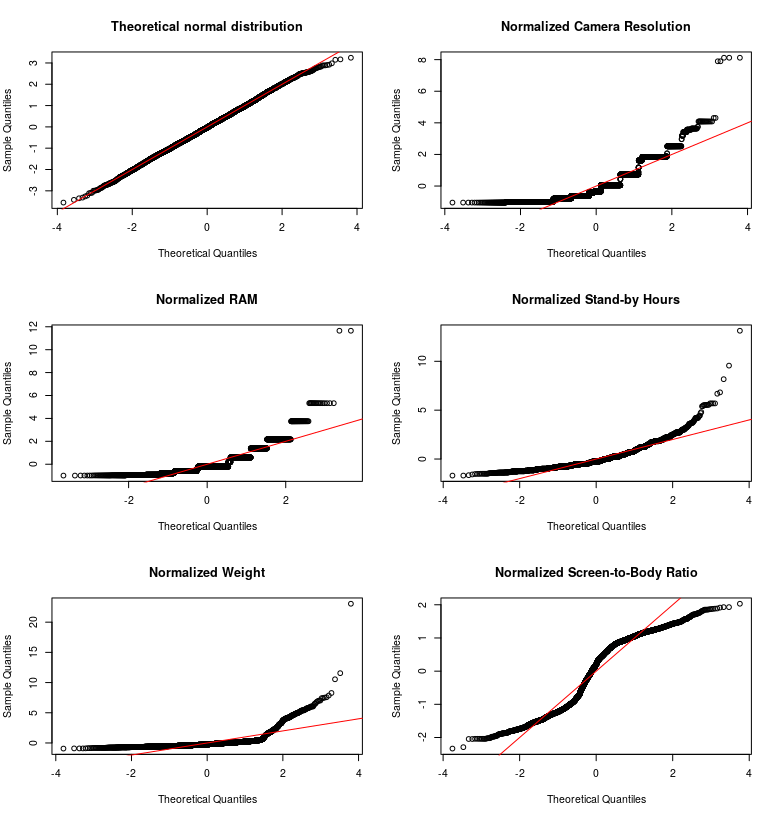
\includegraphics[width=0.85\textwidth]{qqplots.png}
    \caption{Quantile-Quantile Plot of Observations agains Normal Distribution}
    \label{fig:qqplots}
\end{figure}

Shapiro-Wilk test, another powerful normality test, is not powerful enough to handle the data in question with 8020 observation, and thus skipped. As common practice, QQ-plots and/or appropriated Kolmogorov-Simrnov tests are reliable and sufficient to assert on normality, especially provided with the strong test statistics with the underlying data. Further discussion and in-depth statistical researches on normality can be found for example \citeauthor{ghasemi2012normality} (\citeauthor{ghasemi2012normality}).

\section{Statistical Note on Selected Graphs}
\label{app:stats note}

In Figure \ref{fig:screen resolutions}, the dots are observed values (with jitters to improve visualization) from each mo-bile phones in the data set, and the blue curves in both graph indicated the corresponding trend over time, which is achieved through a generalized additive models with integrated smoothness estimation. The graph is achieved with visualization implementation as discussed by Wood \citeyear{wood2001mgcv}.

Due to missing information about system chip, 2786 phones data plotted in Figure \ref{fig:systemchip} plots only counts for 34.7\% of total data collected of mobile phone. Moreover, the system chip market are rather concentrated, with Qualcomm and MediaTek dominate 78.2\% (47.6\% and 30.6\% correspondingly

\end{document}
